\documentclass[17pt,a4paper,landscape]{extarticle}
\usepackage[margin=2.35cm,top=0.12cm,left=1.05cm]{geometry}
\usepackage{amsmath}
\usepackage{amssymb}
\usepackage{tasks}
\usepackage{tikz}
\usepackage{xcolor}
\usepackage[sfdefault,lf]{FiraSans}
\renewcommand{\familydefault}{\sfdefault}
\setlength{\parindent}{0pt}
\pagestyle{empty}
\settasks{label=\textbf{\arabic*.}, label-width=2.2em, item-indent=2.95em, column-sep=2.1cm, after-item-skip=4.9em}
\renewcommand{\arraystretch}{1.15}
\everymath{\displaystyle}

\begin{document}
\sffamily
\boldmath

{\LARGE \textbf{Naming angles --- Excellence}}
\begin{tasks}(3)
\task {In the diagram, give two correct names for the marked angle and one incorrect name.\\[0.4em]
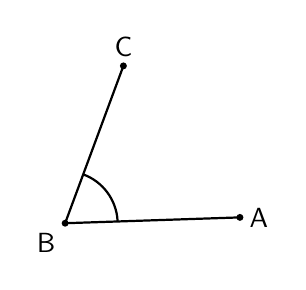
\begin{tikzpicture}[scale=0.74,baseline=(current bounding box.center)]
  \coordinate (B) at (0,0); \coordinate (A) at (3.0,0.1); \coordinate (C) at (1.0,2.7);
  \draw[thick] (B)--(A); \draw[thick] (B)--(C);
  \draw[thick] (0.90,0.04) arc[start angle=3,end angle=70,radius=0.90];
  \fill (A) circle (1.7pt) node[right] {A}; \fill (B) circle (1.7pt) node[below left] {B}; \fill (C) circle (1.7pt) node[above] {C};
\end{tikzpicture}}
\task {In the diagram, give two correct names for the marked angle and one incorrect name.\\[0.4em]
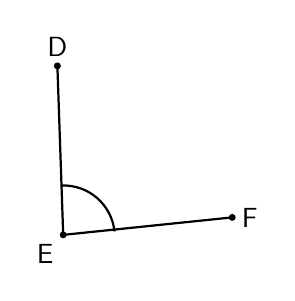
\begin{tikzpicture}[scale=0.74,baseline=(current bounding box.center)]
  \coordinate (E) at (0,0); \coordinate (D) at (-0.1,2.9); \coordinate (F) at (2.9,0.3);
  \draw[thick] (E)--(D); \draw[thick] (E)--(F);
  \draw[thick] (0.88,0.06) arc[start angle=6,end angle=92,radius=0.88];
  \fill (D) circle (1.7pt) node[above] {D}; \fill (E) circle (1.7pt) node[below left] {E}; \fill (F) circle (1.7pt) node[right] {F};
\end{tikzpicture}}
\task {A student says \mbox{$\angle ABC$} and \mbox{$\angle BAC$} are both correct because they use the same three letters. Explain the mistake.}
\task {A student writes \mbox{$\angle XYZ$} when the vertex is \mbox{$Z$}. Rewrite the angle name correctly using the same letters.}
\task {Point \mbox{$Q$} is the vertex. One arm goes through \mbox{$P$} and the other goes through \mbox{$R$}. Write every correct three-letter name for the angle.}
\task {Point \mbox{$N$} is the vertex. One arm goes through \mbox{$M$} and the other goes through \mbox{$L$}. Write every correct three-letter name for the angle.}
\task {Four rays \mbox{$OA$}, \mbox{$OB$}, \mbox{$OC$} and \mbox{$OD$} meet at \mbox{$O$}. Name the angle formed by \mbox{$OA$} and \mbox{$OC$} in two ways.}
\task {Four rays \mbox{$TH$}, \mbox{$TJ$}, \mbox{$TK$} and \mbox{$TL$} meet at \mbox{$T$}. Name the angle formed by \mbox{$TJ$} and \mbox{$TL$} in two ways.}
\task {Decide whether each is correct or incorrect for the same angle with vertex \mbox{$B$}: \mbox{$\angle ABC$}, \mbox{$\angle CBA$}, \mbox{$\angle ACB$}, \mbox{$\angle CAB$}.}
\task {Decide whether each is correct or incorrect for the same angle with vertex \mbox{$M$}: \mbox{$\angle LMN$}, \mbox{$\angle NML$}, \mbox{$\angle LNM$}, \mbox{$\angle MLN$}.}
\task {The angle between rays \mbox{$VX$} and \mbox{$VY$} is called \mbox{$\angle XVY$}. Explain why \mbox{$\angle YVX$} is also correct.}
\task {The angle between rays \mbox{$CD$} and \mbox{$CE$} is called \mbox{$\angle DCE$}. Explain why \mbox{$\angle CDE$} is not correct.}
\task {Create your own labelled angle using points \mbox{$A$}, \mbox{$B$} and \mbox{$C$}. Then write one correct name and one incorrect name.}
\task {Create your own labelled angle using points \mbox{$P$}, \mbox{$Q$} and \mbox{$R$}. Then write two correct names for the same angle.}
\task {What is the one position in a three-letter angle name that can never change if you are naming the same angle? Explain.}
\task {Why do mathematicians usually use three letters instead of one letter to name an angle?}
\end{tasks}

\end{document}
